\subsection{Technologiewahl Anhang} 

\subsubsection{Stimmen verwendeter Frameworks} 

\begin{figure}[H]
	\centering
    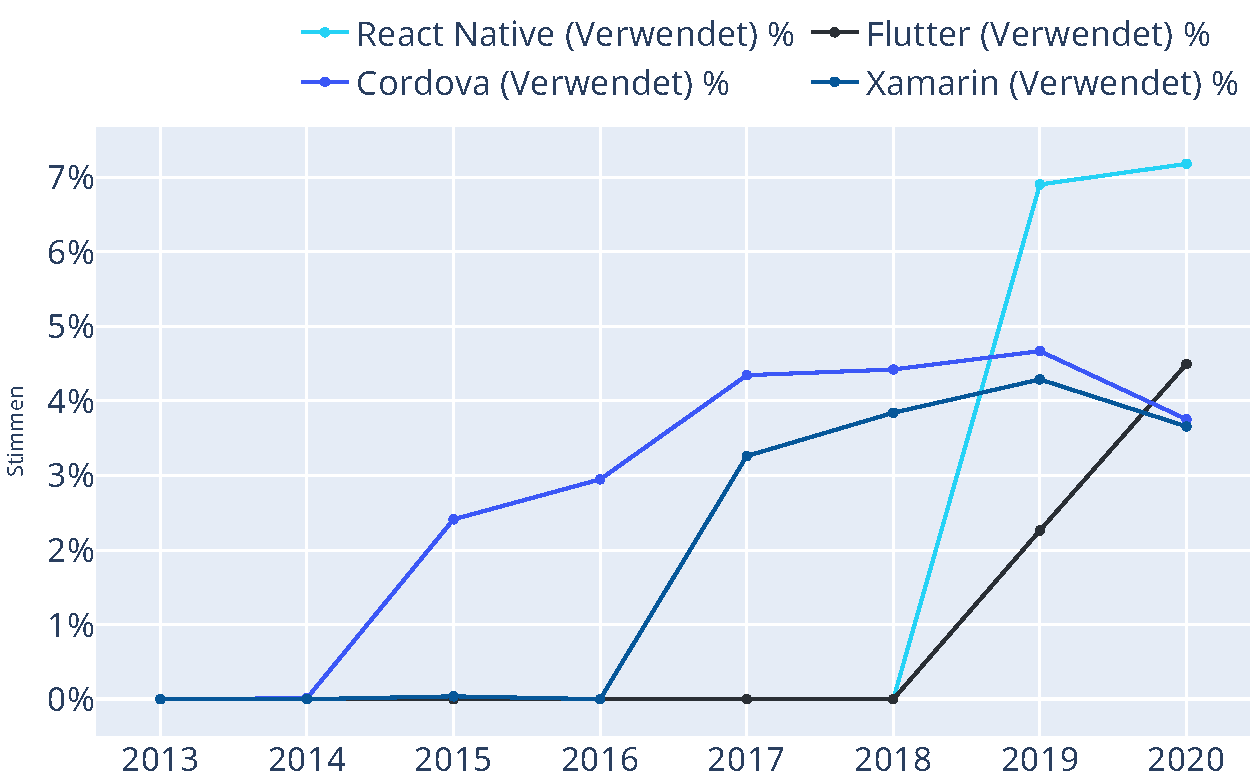
\includegraphics[width=1.0\textwidth]{Charts/Stack Overflow Umfrage/Stimmen verwendeter Frameworks.pdf}
	\caption[Stimmen verwendeter Frameworks]{Stimmen verwendeter Frameworks, Quelle: Eigene Abbildung, Notebook: Charts/Stack Overflow Umfrage/Stack Overflow Umfrage.ipynb}
	\label{fig:StimmenVerwendeter Frameworks}
\end{figure}


\subsubsection{Stimmen gewünschter Frameworks} 

\begin{figure}[H]
	\centering
    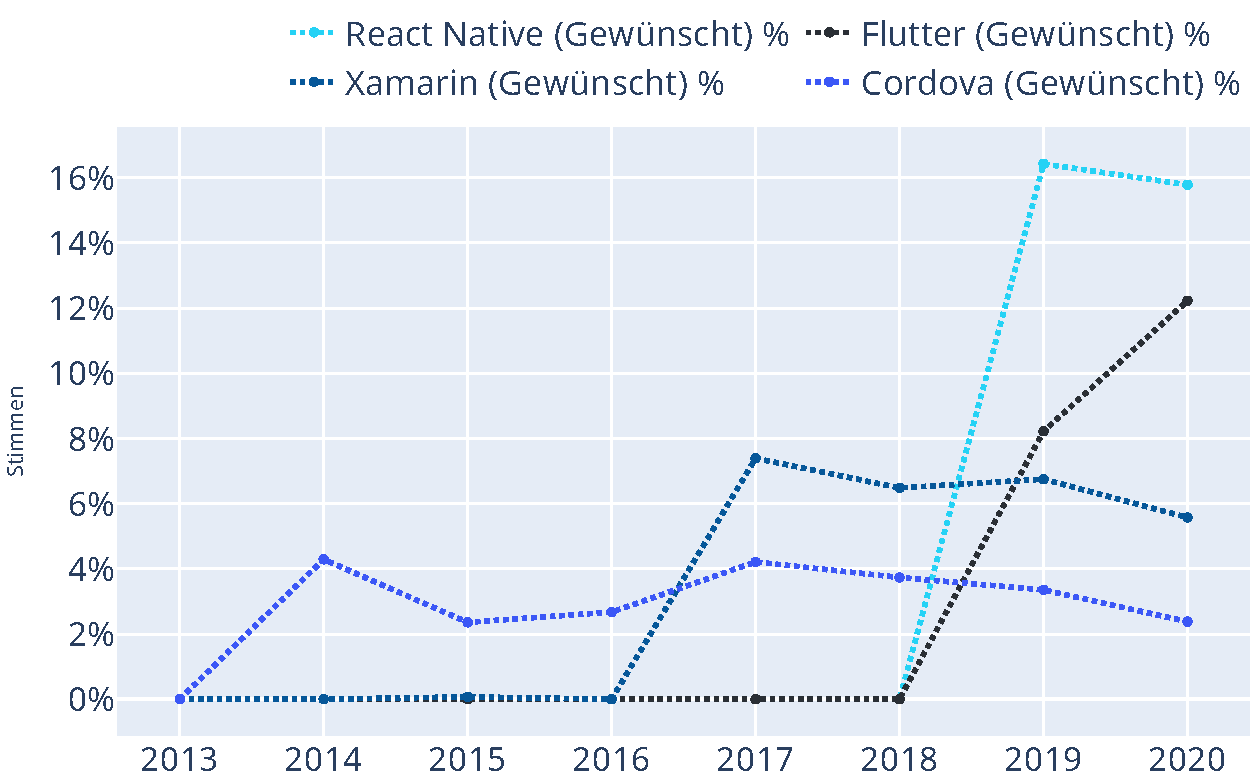
\includegraphics[width=1.0\textwidth]{Charts/Stack Overflow Umfrage/Stimmen gewuenschter Frameworks.pdf}
	\caption[Stimmen gewünschter Frameworks]{Stimmen gewünschter Frameworks, Quelle: Eigene Abbildung, Notebook: Charts/Stack Overflow Umfrage/Stack Overflow Umfrage.ipynb}
	\label{fig:StimmenGewuenschterFrameworks}
\end{figure}


 


\subsection{Vergleich React Native und Flutter Anhang} 



\begin{listing}[h]
  \inputminted[firstline=0] {dart}
  {Quellcode/Vergleich/form-in-flutter/lib/main.dart}
\caption[]{, Quelle: Eigenes Listing, \newline Datei: Quellcode/Vergleich/form-in-flutter/lib/validation.dart}
\label{lst:Schritt1KlasseLetzterStatus}
\end{listing} 



\begin{listing}[h]
  \inputminted[firstline=0] {dart}
  {Quellcode/Vergleich/form-in-flutter/lib/validation.dart}
\caption[]{, Quelle: Eigenes Listing, \newline Datei: Quellcode/Vergleich/form-in-flutter/lib/validation.dart}
\label{lst:Schritt1KlasseLetzterStatus}
\end{listing} 

\begin{listing}[h]
  \inputminted[firstline=0] {dart}
  {Quellcode/Vergleich/form-in-flutter/lib/input.dart}
\caption[]{, Quelle: Eigenes Listing, \newline Datei: Quellcode/Vergleich/form-in-flutter/lib/input.dart}
\label{lst:Schritt1KlasseLetzterStatus}
\end{listing} 

\begin{listing}[h]
  \inputminted[firstline=0] {dart}
  {Quellcode/Vergleich/form-in-flutter/lib/input.dart}
\caption[]{, Quelle: Eigenes Listing, \newline Datei: Quellcode/Vergleich/form-in-flutter/lib/input.dart}
\label{lst:Schritt1KlasseLetzterStatus}
\end{listing} 


\begin{listing}[h]
  \inputminted[firstline=0] {ts}
  {Quellcode/Vergleich/form-in-react-native-the-right-way/App.tsx}
\caption[]{, Quelle: Eigenes Listing, \newline Datei: Quellcode/Vergleich/form-in-react-native-the-right-way/App.tsx}
\label{lst:Schritt1KlasseLetzterStatus}
\end{listing} 

\begin{listing}[h]
  \inputminted[firstline=0] {ts}
  {Quellcode/Vergleich/form-in-react-native-the-right-way/Hero.tsx}
\caption[]{, Quelle: Eigenes Listing, \newline Datei: Quellcode/Vergleich/form-in-react-native-the-right-way/Hero.tsx}
\label{lst:Schritt1KlasseLetzterStatus}
\end{listing} 

\begin{listing}[h]
  \inputminted[firstline=0] {ts}
  {Quellcode/Vergleich/form-in-react-native-the-right-way/validation.tsx}
\caption[]{, Quelle: Eigenes Listing, \newline Datei: Quellcode/Vergleich/form-in-react-native-the-right-way/validation.tsx}
\label{lst:Schritt1KlasseLetzterStatus}
\end{listing} 

\begin{listing}[h]
  \inputminted[firstline=0] {ts}
  {Quellcode/Vergleich/form-in-react-native-the-right-way/components/Form.tsx}
\caption[]{, Quelle: Eigenes Listing, \newline Datei: Quellcode/Vergleich/form-in-react-native-the-right-way/components/Form.tsx}
\label{lst:Schritt1KlasseLetzterStatus}
\end{listing} 

\begin{listing}[h]
  \inputminted[firstline=0] {ts}
  {Quellcode/Vergleich/form-in-react-native-the-right-way/components/Input.tsx}
\caption[]{, Quelle: Eigenes Listing, \newline Datei: Quellcode/Vergleich/form-in-react-native-the-right-way/components/Input.tsx}
\label{lst:Schritt1KlasseLetzterStatus}
\end{listing} 